\documentclass[a4paper,12pt]{article}
\usepackage{graphicx} 			% Para insertar imagenes
\usepackage{indentfirst} 	% Para sangrar párrafos después de secciones
\setlength{\parindent}{1.5cm} 	% Sangría de 1.5 cm
%\renewcommand{\thesubsection}{\alph{subsection}} 	% Para que las subsecciones empiezen por letras minúsculas.
\usepackage{minted} 	% Para insertar código 
\usepackage{float}
\usepackage[spanish, es-tabla]{babel}
\usepackage{tcolorbox} % Para secciones en destacado

\title{Práctica 3: Java RMI }
\author{Ángel Rodríguez Faya}
\date{22 de abril de 2026}

\usepackage{amsmath}
\usepackage{amssymb}

\begin{document}
	
	% --- PÁGINA 1: LA PORTADA ---
	\begin{titlepage}
		\centering
		\vspace*{1cm}
		
		{\huge\bfseries Práctica 3: Java RMI \par}
		\vspace{1.5 cm}
		
		{\Large Desarrollo de Sistemas Distribuidos. Grupo DSD-3. \par}
		\vspace{0.25cm}
		{\Large Grado en Ingeniería Informática \par}
		\vspace{0.25cm}
		{\Large Curso 2025-2026.\par}
		\vspace{0.25cm}
		{\Large ETSIIT. Universidad de Granada.\par}
		\vspace{1 cm}
		
		\noindent % Evita la sangría para que aproveche todo el ancho
		\begin{minipage}[c]{0.55\textwidth}
			% La imagen ocupa el 100% del ancho DE ESTA CAJA (no de la hoja)
			
\includegraphics[width=\linewidth]{./imagenes_necesarias/Logotipo_ETSIIT_Horizontal_color.png}
		\end{minipage}% <--- Este % es importante para que no añada espacios extra
		\hfill % Rellena el espacio en medio empujando las cajas a los extremos
		\begin{minipage}[c]{0.40\textwidth}
			\raggedleft % Alinea esta imagen a la derecha dentro de su caja
			
\includegraphics[width=\linewidth]{./imagenes_necesarias/UGR-LOGO-color.png}
		\end{minipage}
		
		\vspace{0.5 cm}
		
		{\large\bfseries Autor: \par}
		{\large Ángel Rodríguez Faya \par}
		\vspace{0.5cm}
		
		{\large\bfseries Profesor: \par}
		{\large José Ángel Segura Muros \par}
		\vspace{1 cm}
		
		{\large\bfseries Fecha de entrega: \par}
		{\large 24 de abril de 2026\par}
		
	\end{titlepage}
	% El entorno 'titlepage' hace el salto de página automáticamente al cerrar.
	
	% --- PÁGINA 2: EL ÍNDICE ---
	\tableofcontents
	\newpage % <--- Fuerza el salto a la página 3
	
	% --- RESTO DE PÁGINAS:
	
	\section{Introducción}
		En esta tercera práctica vamos a trabajar y aprender el manejo de los mecanismos para implementar programas distribuidos en Java, haciendo uso de su API \textbf{RMI} (\textit{\textbf{R}emote \textbf{M}ethod \textbf{I}nvocation}), que nos permite construir objetos distribuidos. Como entorno de funcionamiento se utilizará la máquina virtual de java (\textit{JVM}, Java Virtual Machine) que sigue un enfoque \textit{“Write Once, Run Anywhere”}, que su traducción viene a ser: “se codifica una vez y se ejecuta en cualquier sitio”), usando este enfoque para que se ejecute en ó por todas partes (\textit{“run everywhere”}).
		
		 Los sistemas RMI se caracterizan porque existe un objeto delegado (que llamaremos \textit{stub)}) que es el encargado de gestionar las invocaciones al objeto remoto, gestionando la serialización y deserialización de los parámetros y valores de retorno. 
		 
		 Las aplicaciones en RMI (denominadas \textbf{aplicaciones de objetos distribuidos})están formadas por dos aplicaciones: el cliente y el servidor. El servidor es el encargado de crear los objetos remotos, hacer accesibles las referencias a dichos objetos remotos y esperar la invocación de métodos sobre dichos objetos remotos por parte de los clientes. Estos, los clientes, obtienen una referencia remota a uno o varios objetos remotos en el servidor e invocan métodos sobre los objetos remotos. RMI proporciona los mecanismos que permiten la comunicació y el intercambio de información entre el cliente y el servidor.
		 
		 A continuación, veremos los tres ejemplos que nos dan en el guion de este práctica, los ejecutaremos y analizaremos que está sucediendo, así como mostrar sus archivos, pues considero que es más cómodo a la hora de corregir, tenerlo todo en un documento (hablo de tener el código fuente de los ejercicios más ejemplos de ejecución), que tener la necesidad de abrir el documento y el editor de código a la vez.
		 
	\section{Parte 1. Ejemplos del guion.}
		
		\subsection{Ejemplo 1. Cliente-Servidor básico.}
			Este ejemplo es una muestra de cómo se realiza una implementación básica de una aplicación Cliente-Servidor en Java RMI. Tenemos un servidor llamado \texttt{Ejemplo} que implementa un método \texttt{escribir\_mensaje(int idProceso)}, que recibe un entero que representa el identificador del proceso (Cliente) que invoca a este método del servidor, y muestra por pantalla dicho identificador. Si se trata del proceso/hebra 0, entonces la duerme 5 segundos y después continua como el resto de procesos.
			
			Veamos cada uno de los archivos que forman este ejemplo. Es importante señalar que \textbf{este código ha sido modificado durante las sesiones de prácticas}, pues se trata de una práctica antigua y hay paquetes/componentes que actualmente están en estado obsoletos.
			
			\subsubsection{\texttt{Ejemplo\_I.java} (La Interfaz Remota)}
				Es la interfaz que define qué métodos del servidor pueden ser llamados por el cliente a través de la red.
				
				Su código es:			
				\inputminted[linenos, frame=lines, fontsize=\footnotesize]{Java}{../codigo/Parte_1/Ejemplo_1/Ejemplo_I.java}
			
			\subsubsection{\texttt{Ejemplo.java} (El Servidor)}
				Implementa la interfaz anteriormente definida, es decir, el método \texttt{escribir\_mensaje}. Esta aplicación está a la espera de recibir peticiones. Aquí se han \textbf{realizado modificaciones}, ya que el \texttt{SecurityManager} del ejemplo está obsoleto (\textit{deprecated}) a partir de Java 17, por lo que se han añadido las clases \texttt{SslRMIClientSocketFactory} y \texttt{SslRMIServerSocketFactory} para que la comunicación vaya cifrada a través de \textbf{SSL/TSL}.
				
				Su código es:			
				\inputminted[linenos, frame=lines, fontsize=\footnotesize]{Java}{../codigo/Parte_1/Ejemplo_1/Ejemplo.java}
			
			\subsubsection{\texttt{Cliente\_Ejemplo.java} (El Cliente)}
				Es el encargado de conectar con el servidor para realizar peticiones. Para ello, se conecta al registro (el \texttt{rmiregistry}) que hace de guía para poder encontrar nuestros objetos, y busca el servidor por su nombre, que sería "Ejemplo\_I". Después se llama al método para escribir el mensaje, pasándole su identificador de proceso como parámetro.
				
				Su código sería el siguiente:
				\inputminted[linenos, frame=lines, fontsize=\footnotesize]{Java}{../codigo/Parte_1/Ejemplo_1/Cliente_Ejemplo.java}
				
			\subsubsection{\texttt{launch.sh} (Script de Ejecución)}
				Nos han proporcionado este script para poder realizar la compilación/ejecución con tan sólo ejecutarlo. Básicamente, lo que hace es crear unos ``certificados digitales'' necesarios para que el SSL funcione en neustra máquina, compilar todos los .java de golpe, lanzar el servidor en segundo plano y por último lanzar dos clientes para que se conecten al servidor, estos clientes tienen como identificadores 0 y 3, respectivamente.
			
				\inputminted[linenos, frame=lines, fontsize=\footnotesize]{Shell}{../codigo/Parte_1/Ejemplo_1/launch.sh}
			
			\subsubsection{Ejemplo de compilación y ejecución del ejemplo 1.}
				En primer lugar, debemos dar permiso de ejecución al script. Para ello abrimos una terminal y ejecutamos el siguiente comando:
				
				\begin{center}
					\fbox{\texttt{\$ chmod u+x launch.sh}}
				\end{center}
				
				Después, ejecutamos el script con el siguiente comando:
				
				\begin{center}
					\fbox{\texttt{\$ ./launch.sh}}
				\end{center}
				
				A continuación, muestro una imagen con la salida de la ejecución:
				
				\begin{figure}[H]
					\centering
					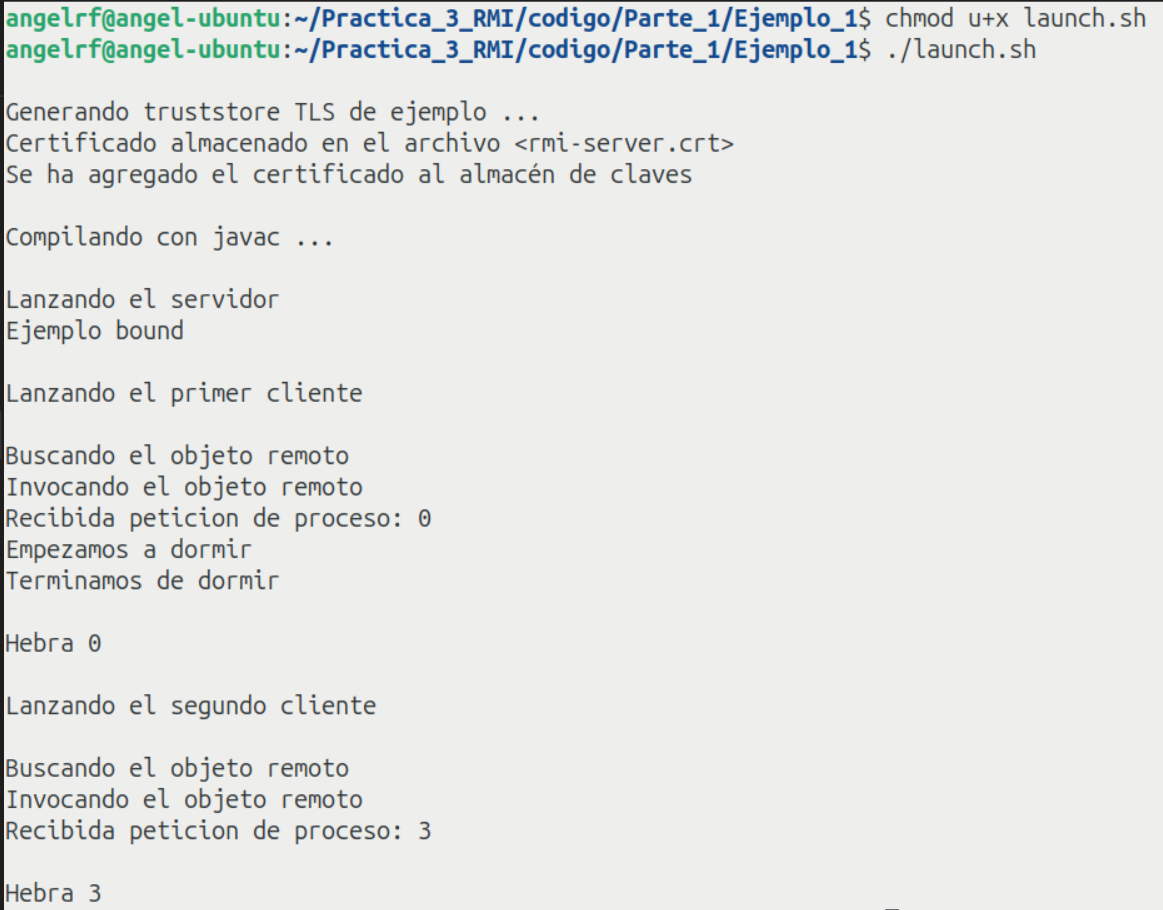
\includegraphics[width=1\linewidth]{./imagenes_necesarias/salida_ejemplo_1.png}
					\caption{Ejecución del ejemplo 1}
					\label{fig:ejecucion_ejemplo1}
				\end{figure}
				
				Como podemos observar en la salida, se compilan todos los archivos, se lanza el servidor y se muestra el mensaje \texttt{"Ejemplo bound"}, que nos indica que el objeto remoto ya puede ser invocado por los clientes.
				Después se lanza el cliente 0. Este busca el objeto remoto y lo invoca. El método de escribir mensaje en el servidor recibe la petición mostrando ese mensaje con el id del proceso cliente. Como se trata del proceso 0, lo pone a dormir 5 segundos. Pasado ese tiempo, muestra el mensaje de que ha terminado de dormir e imprime rl mensaje de hebra con el id de nuevo, y ya termina.
				Finalmente se lanza el cliente con id 3 (aunque no se lanza después de que termine la hebra 0, si no que\textbf{ se lanza la hebra 3 mientras la hebra 0 duerme} ).De nuevo, este cliente busca el objeto remoto y lo invoca. Llama al método para escribir mensaje, este muestra que le ha llegado la petición mostrando su id.

		\subsection{Ejemplo 2. Multihebra.}

				
	
	
\end{document}